\documentclass{amsart}
\usepackage{hyperref,tikz,pgfplots,tikz-cd,amssymb}
\tikzset{%https://tex.stackexchange.com/questions/620408/how-can-i-draw-2-tikz-rectangular-grids-side-by-side
  pics/matrix/.style n args={5}{% rows, columns, text above, text below, text left (or symbol)
    code={%
      \begin{scope}[y=-1cm,scale=0.5]
        \draw    (0,0) grid (#2,#1);
        \node at (0.5*#2,-0.5)   {#3};
        \node at (0.5*#2,#1+0.5) {#4};
        \node at (-0.5,0.5*#1)   {#5};
      \end{scope}     
    }},
}

\begin{document}

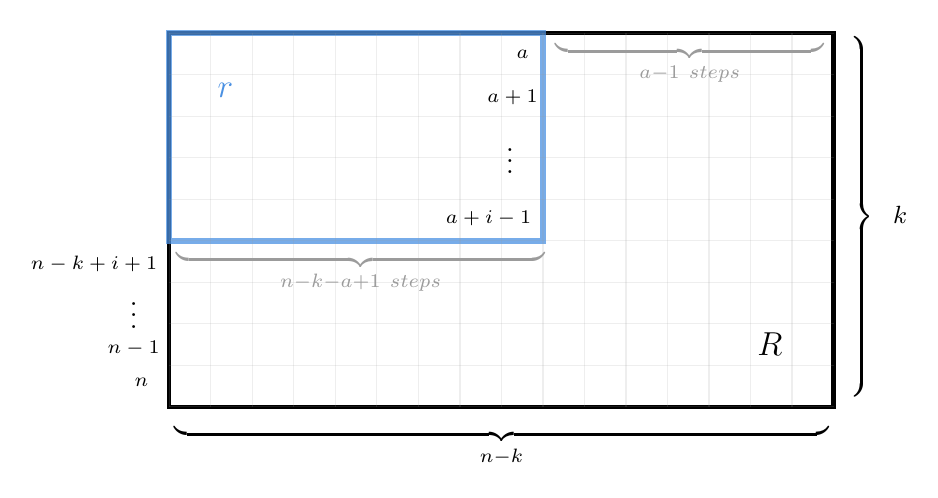
\begin{tikzpicture}[x=0.75pt,y=0.75pt,yscale=-1,xscale=1]

\draw  [color={rgb, 255:red, 0; green, 0; blue, 0 }  ,draw opacity=1 ][line width=1.5]  (146.67,70) -- (466.67,70) -- (466.67,250) -- (146.67,250) -- cycle ;
\draw  [color={rgb, 255:red, 74; green, 144; blue, 226 }  ,draw opacity=0.75 ][line width=2.25]  (146.67,70) -- (326.67,70) -- (326.67,170) -- (146.67,170) -- cycle ;
\draw  [draw opacity=0] (146.67,70) -- (466.67,70) -- (466.67,250) -- (146.67,250) -- cycle ; \draw  [color={rgb, 255:red, 155; green, 155; blue, 155 }  ,draw opacity=0.17 ] (146.67,70) -- (146.67,250)(166.67,70) -- (166.67,250)(186.67,70) -- (186.67,250)(206.67,70) -- (206.67,250)(226.67,70) -- (226.67,250)(246.67,70) -- (246.67,250)(266.67,70) -- (266.67,250)(286.67,70) -- (286.67,250)(306.67,70) -- (306.67,250)(326.67,70) -- (326.67,250)(346.67,70) -- (346.67,250)(366.67,70) -- (366.67,250)(386.67,70) -- (386.67,250)(406.67,70) -- (406.67,250)(426.67,70) -- (426.67,250)(446.67,70) -- (446.67,250) ; \draw  [color={rgb, 255:red, 155; green, 155; blue, 155 }  ,draw opacity=0.17 ] (146.67,70) -- (466.67,70)(146.67,90) -- (466.67,90)(146.67,110) -- (466.67,110)(146.67,130) -- (466.67,130)(146.67,150) -- (466.67,150)(146.67,170) -- (466.67,170)(146.67,190) -- (466.67,190)(146.67,210) -- (466.67,210)(146.67,230) -- (466.67,230)(146.67,250) -- (466.67,250) ; \draw  [color={rgb, 255:red, 155; green, 155; blue, 155 }  ,draw opacity=0.17 ]  ;

% Text Node
\draw (312.67,77) node [anchor=north west][inner sep=0.75pt]  [font=\scriptsize] [align=left] {$\displaystyle a$};
% Text Node
\draw (307.67,116.33) node [anchor=north west][inner sep=0.75pt]   [align=left] {$\displaystyle \vdots $};
% Text Node
\draw (278.67,154) node [anchor=north west][inner sep=0.75pt]  [font=\scriptsize] [align=left] {$\displaystyle a+i-1$};
% Text Node
\draw (298.67,96) node [anchor=north west][inner sep=0.75pt]  [font=\scriptsize] [align=left] {$\displaystyle a+1$};
% Text Node
\draw (78.67,176) node [anchor=north west][inner sep=0.75pt]  [font=\scriptsize] [align=left] {$\displaystyle n-k+i+1$};
% Text Node
\draw (126.33,190.67) node [anchor=north west][inner sep=0.75pt]   [align=left] {$\displaystyle \vdots $};
% Text Node
\draw (115.67,217) node [anchor=north west][inner sep=0.75pt]  [font=\scriptsize] [align=left] {$\displaystyle n-1$};
% Text Node
\draw (128.67,235) node [anchor=north west][inner sep=0.75pt]  [font=\scriptsize] [align=left] {$\displaystyle n$};
% Text Node
\draw (147.67,257.1) node [anchor=north west][inner sep=0.75pt]   [align=left] {$\displaystyle \underbrace{\ \ \ \ \ \ \ \ \ \ \ \ \ \ \ \ \ \ \ \ \ \ \ \ \ \ \ \ \ \ \ \ \ \ \ \ \ \ \ \ \ \ \ \ \ \ \ \ \ \ \ \ \ \ \ \ \ \ \ \ \ \ \ \ \ \ \ \ \ \ \ }_{n-k}$};
% Text Node
\draw (480.08,158.41) node  [rotate=-270] [align=left] {$\displaystyle \underbrace{\ \ \ \ \ \ \ \ \ \ \ \ \ \ \ \ \ \ \ \ \ \ \ \ \ \ \ \ \ \ \ \ \ \ \ \ \ \ \ }$};
% Text Node
\draw (494.17,152) node [anchor=north west][inner sep=0.75pt]  [font=\small] [align=left] {$\displaystyle k$};
% Text Node
\draw (331.67,72.6) node [anchor=north west][inner sep=0.75pt]  [color={rgb, 255:red, 155; green, 155; blue, 155 }  ,opacity=1 ] [align=left] {$\displaystyle \underbrace{\ \ \ \ \ \ \ \ \ \ \ \ \ \ \ \ \ \ \ \ \ \ \ \ \ \ \ \ \ }_{a-1\ steps}$};
% Text Node
\draw (148.67,173) node [anchor=north west][inner sep=0.75pt]  [color={rgb, 255:red, 155; green, 155; blue, 155 }  ,opacity=1 ] [align=left] {$\displaystyle \underbrace{\ \ \ \ \ \ \ \ \ \ \ \ \ \ \ \ \ \ \ \ \ \ \ \ \ \ \ \ \ \ \ \ \ \ \ \ \ \ \ \ }_{n-k-a+1\ steps}$};
% Text Node
\draw (168.67,93) node [anchor=north west][inner sep=0.75pt]  [font=\large,color={rgb, 255:red, 74; green, 144; blue, 226 }  ,opacity=1 ] [align=left] {$\displaystyle r$};
% Text Node
\draw (428.67,213) node [anchor=north west][inner sep=0.75pt]  [font=\large] [align=left] {$\displaystyle R$};


\end{tikzpicture}

\end{document}